\section{Umsetzung}
In diesem Kapitel wird die Vorgehensweise der zuvor beschriebenen Problemstellungen erörtert.

\subsection{Aufbau der Testumgebung}




\subsubsection{Aufsetzen eines Nagios-Test-Systems}
Da die einzelnen Überwachungselemente in der Überwachungssoftware Nagios nach und nach eingetragen (/ definiert / assoziiert / verbunden) werden müssen, ist ein häufiges Neustarten der Nagios Anwendung notwendig, damit die neuen Konfigurationsdateien übernommen werden.

Damit dies nicht auf dem produktiven Nagios-Server durchgeführt werden muss, wird ein Nagios-Testserver für diesen Zwecks eingesetzt.

\subsubsection{Bilddatenbank als VM}
Für die Simulation der verschiedenen Fehlerzuständen der einzelnen Überwachungselemente wird eine virtuelle Maschine mit einer \gls{OracleUCM} Prototypinstallation, die extra als Entwicklungsplattform erstellt wurde, verwendet.


\subsection{Einrichten des Windows Agenten}
\begin{itemize}
\item Port ändern -> RPC
\item Verschlüsselung durch PW und/oder Algo
\item Hinzufügen der Plugins
\item Bsp Aufruf aktiver Check
\end{itemize}

.Net 2.0 Framework essentiell
NC\_Net installieren
nagios server ip zur sicherheit angeben
port ändern
pw hinzufügen
-> dienst starten

test vom nagios host:

\begin{lstlisting}[captionpos=b, caption=Aufruf eines aktiven Checks, label=activecheckexample, breaklines = true]
root@iwrpaul:/usr/local/nagios/libexec# ./check_nc_net -H secret.kit.edu -p 123456 -s secret -v RUNSCRIPT -l check_uname.exe
Operating System OK - Microsoft(R) Windows(R) Server 2003 Standard Edition Service Pack 2
\end{lstlisting}

Das auf dem Nagios Server liegende Script \pictext{check\_nc\_net} stellt eine Verbindung zum angegebenen Server her und führt die mit dem Parameter \pictext{l} angegebene Datei aus. Dafür muss sich diese Datei in dem Script Verzeichnis des NC\_Net befinden.


Danach command definition hinzufügen, weil PW und Port verändert wurde:
\begin{lstlisting}[captionpos=b, caption=Nagios-Befehls Definition für den Host, label=activecheckexample, breaklines = true, language=sh]
# 'check_nt_bdb' command definition
#	_NSCLIENT_PORT	13599
#	_NSCLIENT_PW	KAnqloaQk
#
define command{
    command_name    check_nc_net_bdb
	command_line 	/usr/lib/nagios/plugins/check_nc_net -H $HOSTNAME$ -p 13599 -s KAnqloaQk -v $ARG1$
        }
\end{lstlisting}

Danach
\begin{itemize}
\item Logfiles check.exe 
\item batchloader.exe script
\end{itemize}


\subsection{Überprüfen der Prozesse und Services}
\begin{itemize}
\item Prozesse
\item Services
\item Bsp Aufruf
\end{itemize}

\subsection{Umsetzung der Funktionlitätstest}
\begin{itemize}
\item batchloader + .blo Dateien
\item einloggen mit lokalem und ads benutzer
\end{itemize}



\subsection{Auswertung der Logs + Stopwörterdefinition}
\begin{itemize}
\item check\_logfiles
\item check\_logfiles cfg file inkl. Rotation
\end{itemize}

\subsection{Benutzersimulation}
\gls{SOA} steht für Service-Oriented Architecture und benutzt das Simple Object Access Protocol (\gls{SOAP}), welches ein \gls{XML}-basierendes Protokoll zur Ausführung von Programmen / Befehle auf entfernten Rechnern ist.

\begin{itemize}
\item \url{http://www.w3schools.com/soap/default.asp} Web Services und SOAP
\item \url{http://www.w3schools.com/wsdl/wsdl_summary.asp} WSDL
\item max attempts bei Search erhöhen, da Auslastung der InboundRef -> möglichst keine/geringe False Positives -> auf Ausblick verweisen, Rahmenbedingungen müssen im Feld in der Praxis erst noch gefunden werden
\end{itemize}

\begin{figure}[ht]
	\centering
	   \fbox{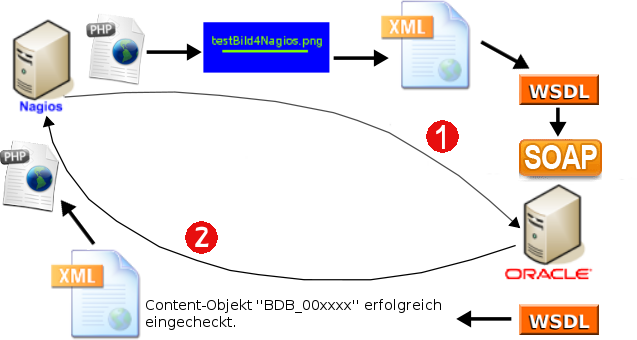
\includegraphics[width=0.9\textwidth]{bilder/wsdl.png}}
		\caption{Ablauf der Benutzersimulation}
		\label{usersim}
\end{figure}
%
\begin{figure}[ht]
	\centering
	   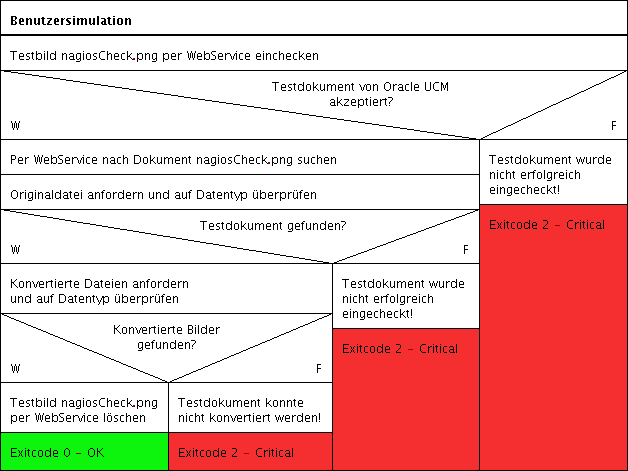
\includegraphics[width=0.9\textwidth]{bilder/Benutzersimulation.png}
		\caption{Ablauf der Benutzersimulation}
		\label{user-sim}
\end{figure}



